%% Les annexes :-)

\section{Diagramme du système multi agent}

\label{diagSMA}
\begin{center}
  \includegraphics[angle=90,width=0.9\textwidth]{img/diagSMA.png}
\end{center}

\section{Vue générale du diagramme de classe}

\label{diag_class}
\begin{center}
  \includegraphics[angle=90,width=0.75\textwidth]{img/class_diag/diag.pdf}
\end{center}

\section{Diagramme de classe détaillé}

\label{diag_class_detail}

\begin{center}
  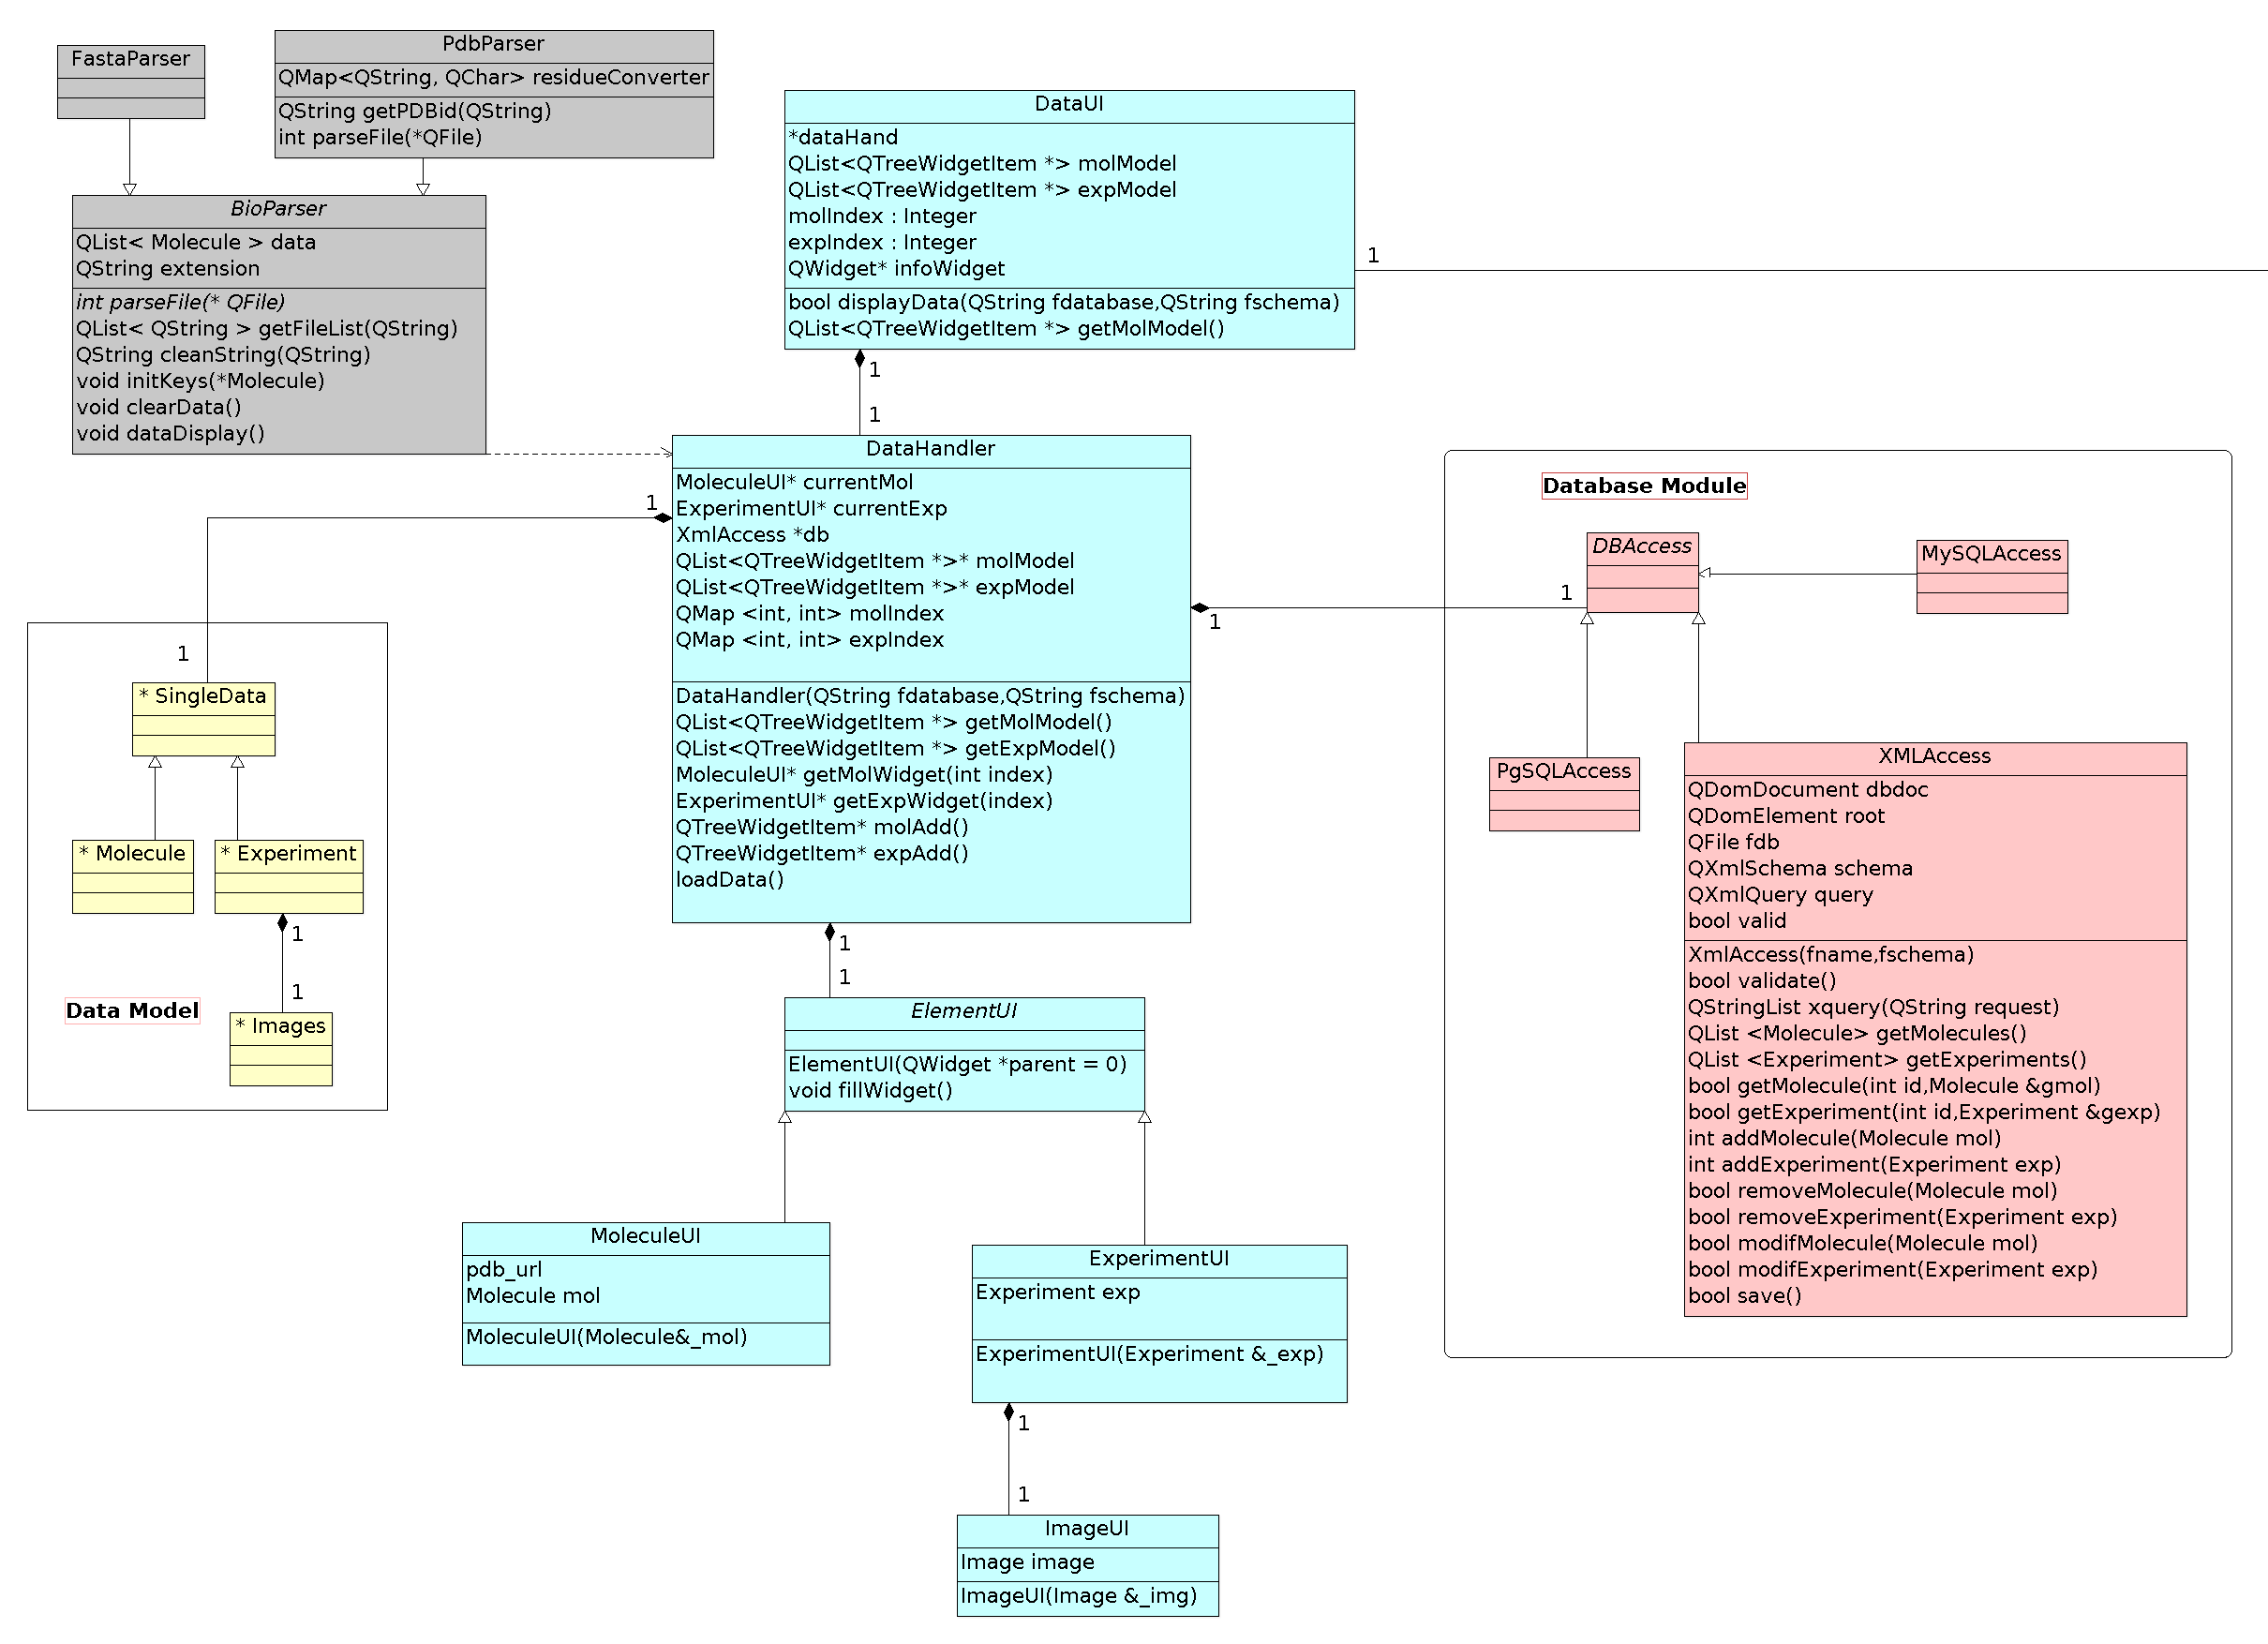
\includegraphics[angle=90,width=1\textwidth]{img/class_diag/diag1.png}
\end{center}
\newpage

\begin{center}
  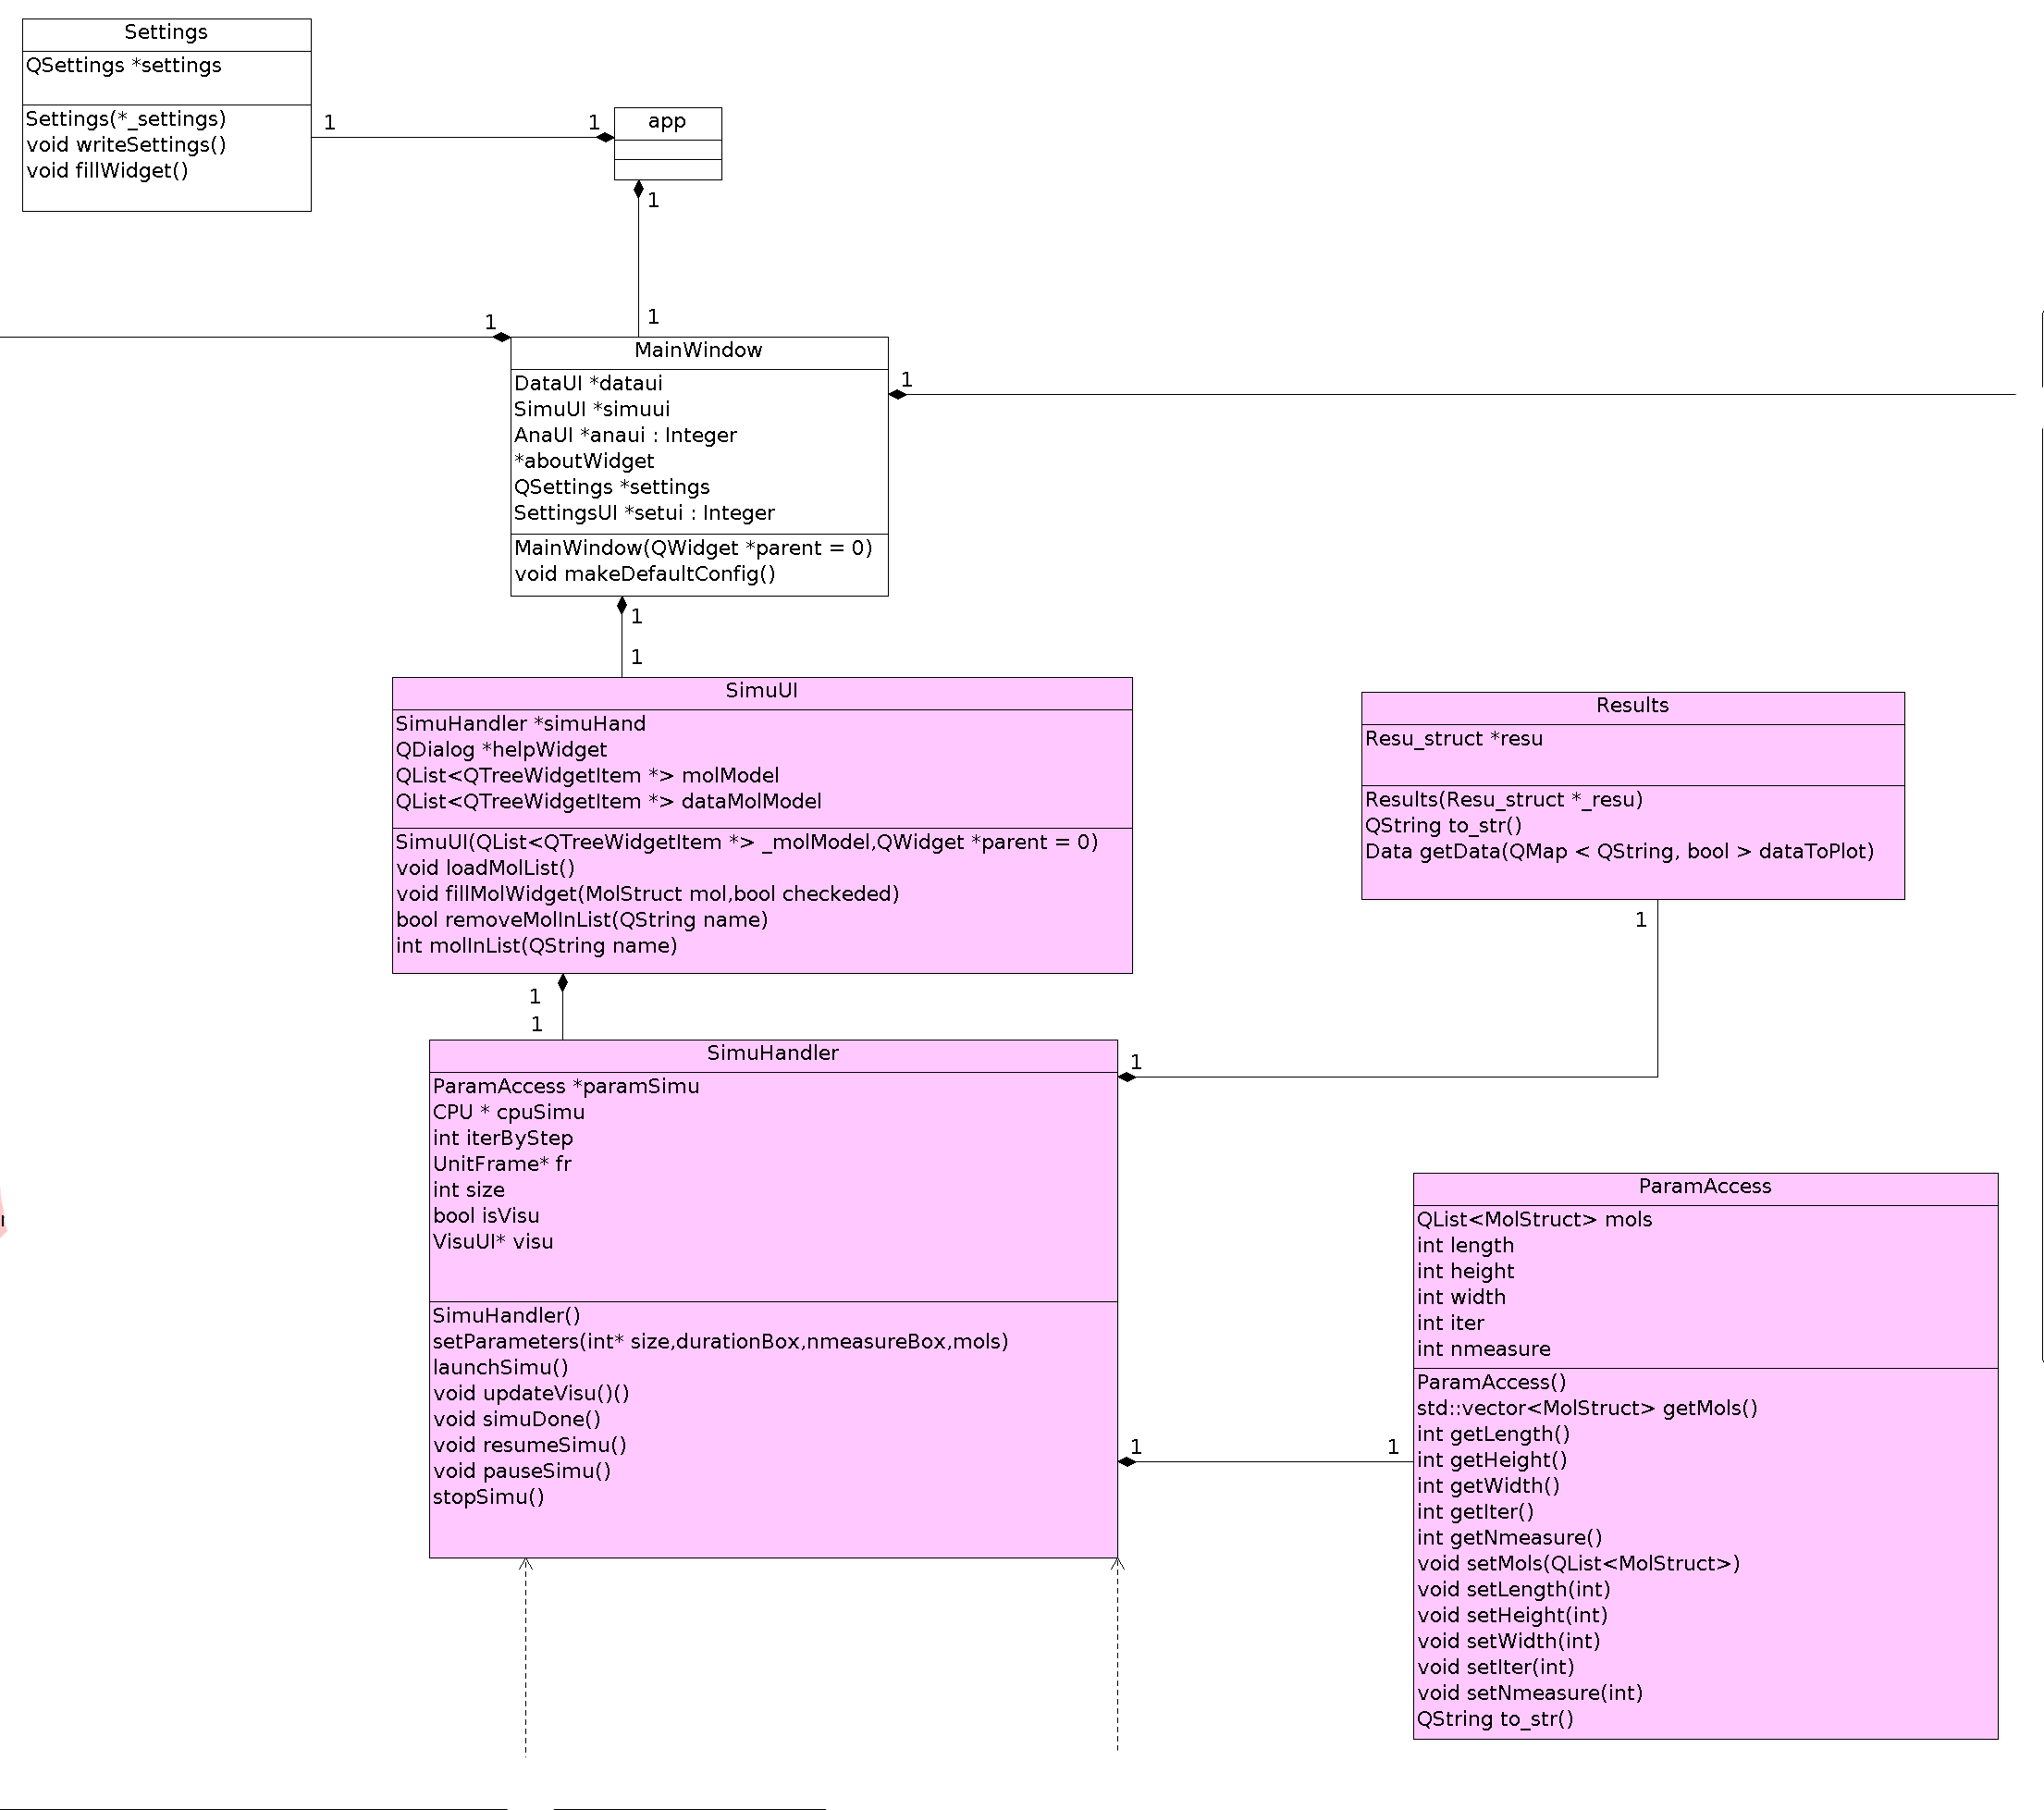
\includegraphics[angle=90,width=0.8\textwidth]{img/class_diag/diag2.png}
\end{center}
\newpage

\begin{center}
  \includegraphics[angle=90,width=0.8\textwidth]{img/class_diag/diag3.png}
\end{center}
\newpage

\begin{center}
  \includegraphics[angle=90,width=0.9\textwidth]{img/class_diag/diag5.png}
\end{center}
\newpage

\begin{center}
  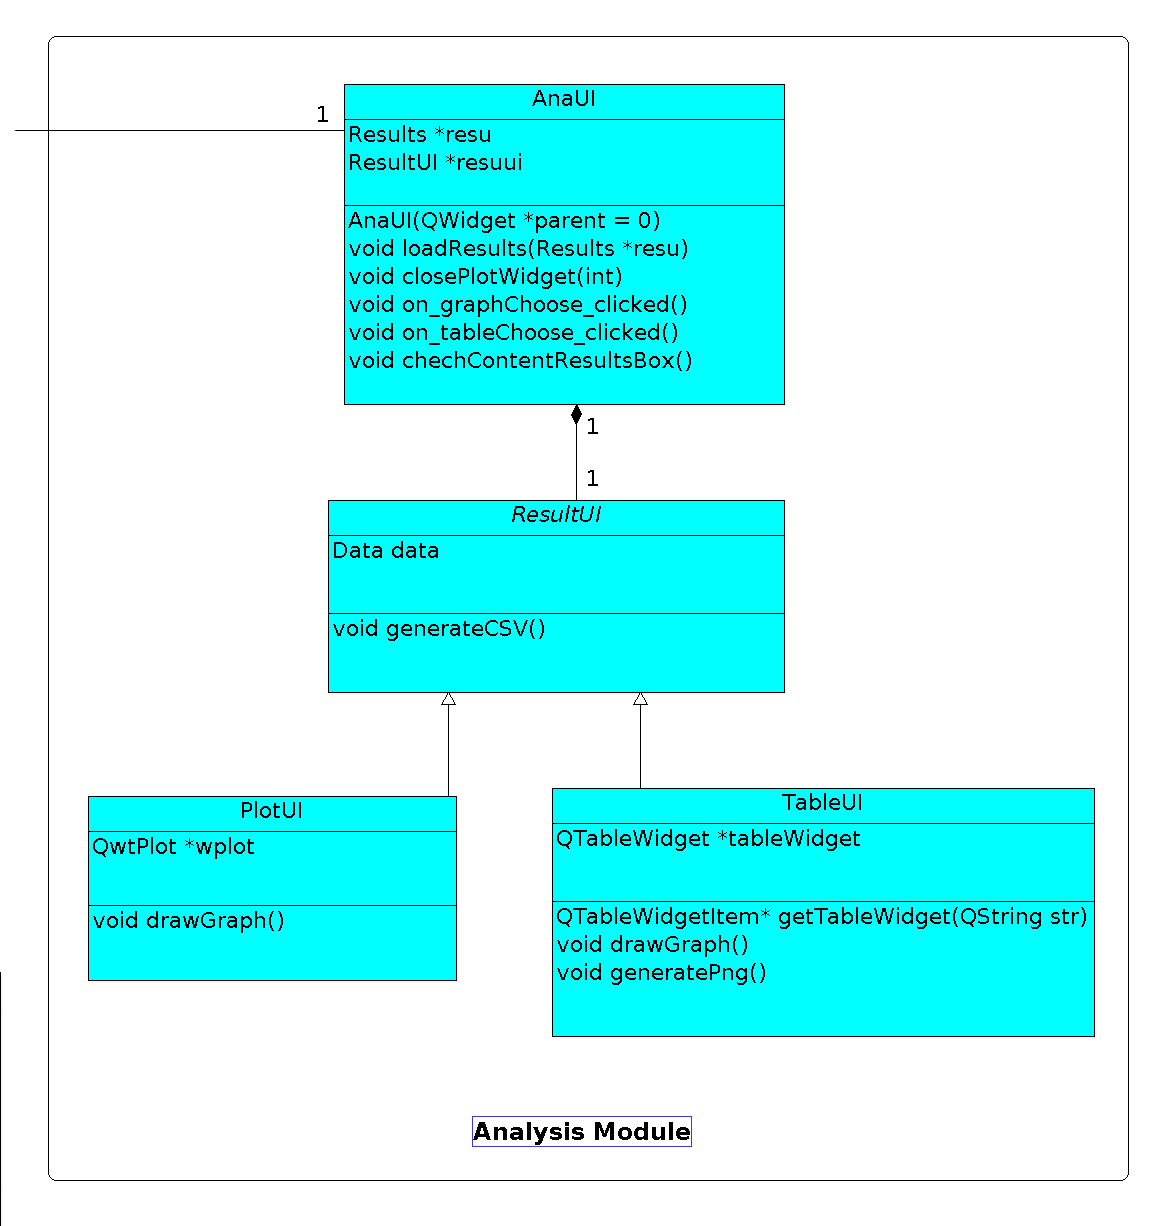
\includegraphics[angle=90,width=1\textwidth]{img/class_diag/diag4.png}
\end{center}

% \section{Représentation métabolique manuelle et automatique}
% \label{repauto}
% \bigskip
% \image{real/norm_before}{Représentation manuelle}{1}
% \imageext{real/norm_after.pdf}{Représentation automatique}{1}
% \imageext{real/norm_after2.pdf}{Représentation automatique à partir du fichier SBML BIOMD0000000019 de BioModels}{0.45}

% \section{Structure du fichier paramètre}
% \label{structparam}
% \bigskip
% \begin{figure}[H]
%   \includegraphics[angle=90,width=1\textwidth]{img/real/carte_schema}
%   \caption{Structure sous forme d'un arbre, du fichier de paramètre.}
% \end{figure}

%%% Local Variables: 
%%% mode: latex
%%% TeX-master: "../main"
%%% End: 
